% Section content template for individual Educative lessons
% This file contains the actual content for a specific section
% Generated from Educative API section content

% Section: Data Replication
% Section ID: 5241733675220992
% Section Slug: data-replication
% Generated: 2025-12-06T21:14:42.122814

Data is a valuable asset for an organization because it drives the entire business.
\\
Data provides critical business insights into what's important and what needs to be changed. Organizations also need to securely save and serve their clients' data on demand. Timely access to the required data under varying conditions (including increasing reads and writes, disk and node failures, network and power outages, and others) is necessary to successfully run an online business.
\\
We need the following characteristics from our data store:

\begin{itemize}
\item
\protect\phantomsection\label{riSSwQqPf5Gab0sbmHKzN}
Availability under faults (failure of one or more disks, nodes, network, or power outages).
\item
\protect\phantomsection\label{VsmW85br7UM5doZ6aAocv}
Scalability (with increasing reads, writes, and other operations).
\item
\protect\phantomsection\label{zuM-RoCRLz1x35D-neerU}
Performance (low latency and high throughput for the clients).
\end{itemize}
\\
It's challenging, or even impossible, to achieve the above characteristics on a single node.

\subsection{Replication}\label{C_jDLaBiATQCKHvgJeaj4}

\textbf{Replication} refers to keeping multiple copies of the data at various nodes (preferably geographically distributed) to achieve availability, scalability, and performance. In this lesson, we assume that a single node is enough to hold our entire data. We won't use this assumption while discussing the partitioning of data in multiple nodes. Often, the concepts of replication and partitioning go together.
\\
Replication provides several key benefits for distributed systems: - Keeps data geographically close to your users, thus reducing access latency. - Allows the system to continue working even if some of its parts have failed, thus increasing availability. - Scales out the number of machines that can serve read queries, thus increasing read throughput.
\\
However, with many benefits, like availability, replication comes with its complexities. Replication is relatively simple if the replicated data doesn't require frequent changes. The main problem in replication arises when we have to maintain changes in the replicated data over time.
\\
If the data that you are replicating does not change over time, then the replication process is a one-time thing. Frequently changing data is a real challenge; it requires careful thinking about concurrency and all the things that can go wrong so that we can deal with the consequences of those faults.
\\
Additional complexities that could arise due to replication are as follows:

\begin{itemize}
\tightlist
\item
How do we keep multiple copies of data consistent with each other?
\item
How do we deal with failed replica nodes?
\item
Should we replicate synchronously or asynchronously?

\begin{itemize}
\tightlist
\item
How do we deal with replication lag in case of asynchronous replication?
\end{itemize}
\item
How do we handle concurrent writes?
\item
What consistency model needs to be exposed to the end programmers?
\end{itemize}
\\
We'll explore the answer to these questions in this lesson.

\begin{figure}[htbp]
 \centering
 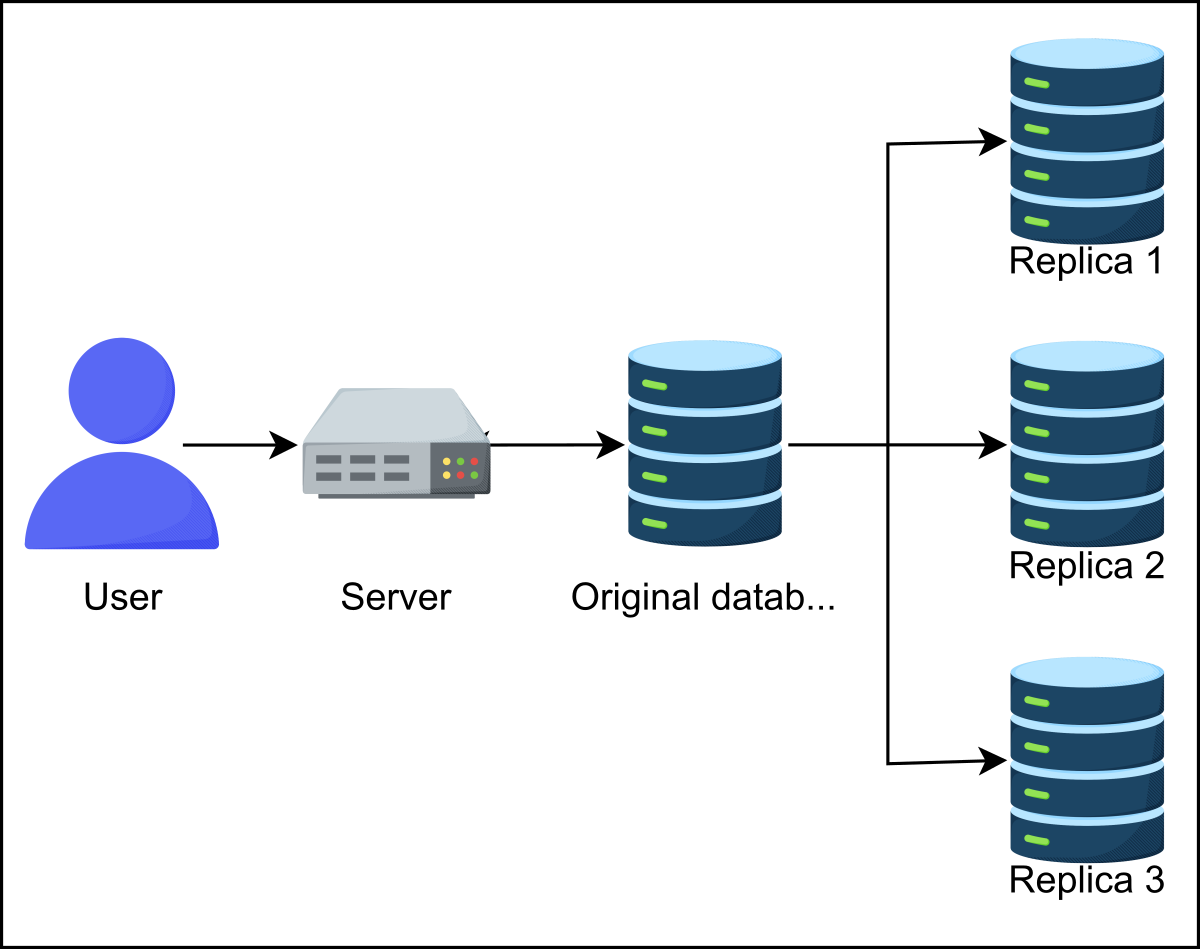
\includegraphics[width=0.5\textwidth]{Images/chapter_9/section_5241733675220992/5382667397103616.png}
 \caption{Replication in action}
\end{figure}

Before we explain the different types of replication, let's understand the synchronous and asynchronous approaches of replication.

\subsection{Synchronous vs. asynchronous replication}\label{GLkDFWuW8EO62L_xGeDY7}
\\
There are two ways to disseminate changes to the replica nodes:

\begin{itemize}
\item
\protect\phantomsection\label{n3wGqcxp5WMm-hlRT_9ut}
Synchronous replication
\item
\protect\phantomsection\label{SKsJFBXGdVxareh7eKpkS}
Asynchronous replication
\end{itemize}
\\
\\
In \textbf{synchronous replication}, the primary node waits for acknowledgments from secondary nodes to confirm that the data has been updated.
\\
After receiving acknowledgment from all secondary nodes, the primary node reports success to the client. In asynchronous replication, the primary node doesn't wait for acknowledgments from the secondary nodes and reports success to the client after updating itself. The advantage of synchronous replication is that all secondary nodes are completely up-to-date with the primary node.
\\
However, there's a disadvantage to this approach.
\\
If one of the secondary nodes fails to acknowledge due to a network failure or fault, the primary node will be unable to acknowledge the client until it receives a successful acknowledgment from the crashed node. This causes high latency in the response from the primary node to the client. On the other hand, the advantage of asynchronous replication is that the primary node can continue its work even if all the secondary nodes are down.
\\
However, if the primary node fails, the writes that weren't copied to the secondary nodes will be lost.
\\
Often, leader-based replication is configured to be completely asynchronous. In this case, if the master fails and is not recoverable, any writes that have not yet been replicated to slaves are lost. This means that a write is not guaranteed to be durable, and weakening durability is a significant trade-off that must be carefully considered. The above paragraph explains a trade-off between data consistency and availability when different components of the system can fail.

\begin{figure}[htbp]
 \centering
 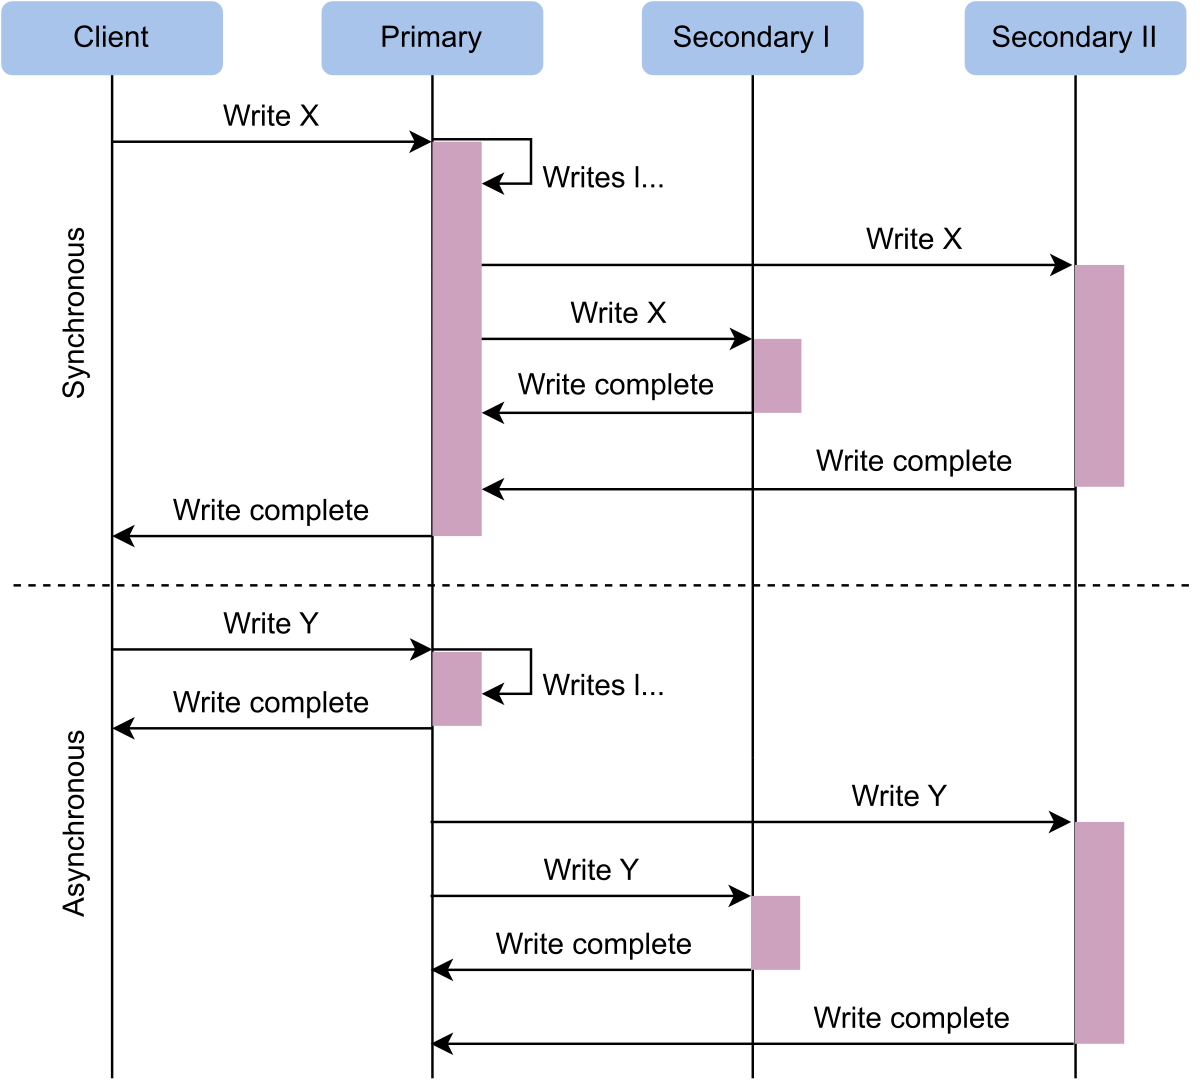
\includegraphics[width=0.5\textwidth]{Images/chapter_9/section_5241733675220992/5769714890702848.png}
 \caption{Synchronous versus asynchronous replication}
\end{figure}

\begin{center}\rule{0.5\linewidth}{0.5pt}\end{center}
\\
Let's assess our understanding of the content provided in this lesson with this question:
\\
Imagine you're leading the database architecture for a real-time financial trading platform that operates globally. The platform demands extremely low-latency data updates to ensure traders receive up-to-the-moment information for making split-second decisions.
\\
The existing database infrastructure is struggling to meet the stringent latency requirements.
\\
In this case, the low latency is paramount, and a certain degree of eventual consistency is acceptable. Which one of the following two choices would you recommend for data updates in the database, and why?

\begin{itemize}
\item
Synchronous updates
\item
Asynchronous updates
\end{itemize}
\\
Provide your answer in this interactive widget:

\textbf{Question:}

Choose the correct option by providing a valid reason below

\textbf{Reference Answer:}

In scenarios where achieving low latency is of utmost importance and accepting eventual consistency is feasible, the recommended choice is asynchronous replication. Unlike synchronous replication, which guarantees data consistency by waiting for acknowledgments from secondary nodes before confirming success, asynchronous replication prioritizes the primary node's continuous operation. It reports success to the client after updating itself, effectively reducing latency. The potential latency introduced by synchronous replication, especially if a secondary node fails to acknowledge, is mitigated by the asynchronous approach, making it a favorable option for environments where swift and continuous data updates are critical.

\subsection{Data replication models}\label{uxqqL7juh-EpNn27TqMAS}
\\
If the data that you are replicating does not change over time, then the replication process is a one-time thing. Frequently changing data presents a significant challenge; it requires careful consideration of concurrency and potential issues to mitigate the consequences of those faults.
\\
At a minimum, we need to address unavailable nodes, network interruptions, and silent data corruption resulting from application bugs.
\\
Here are the following algorithms for replicating changes across nodes:

\begin{itemize}
\item
\protect\phantomsection\label{4RbFiAnJnk9YQVonQjVrH}
Single leader or primary-secondary, or master-slave replication
\item
\protect\phantomsection\label{5nr5oInKjShcSWU3H9sAM}
Multi-leader replication
\item
\protect\phantomsection\label{7Y6suULJlqI7RD9Q7PNd0}
Peer-to-peer or leaderless replication
\end{itemize}

\subsubsection{Single leader/primary-secondary replication}\label{pYxw4WM7PLhUF8M57wxrZ}
\\
In \textbf{primary-secondary replication,} data is replicated across multiple nodes.
\\
One node is designated as the primary. It's responsible for processing any writes to data stored on the cluster. It also sends all the writes to the secondary nodes and keeps them in sync. Primary -secondary replication is appropriate when our workload is read-heavy.
\\
To better scale with increasing readers, we can add more followers and distribute the read load across the available followers.
\\
However, replicating data to many followers can create a primary bottleneck. Additionally , primary-secondary replication is inappropriate if our workload is write-heavy. Another advantage of primary-secondary replication is that it's read-resilient.
\\
Secondary nodes can still handle read requests in the event of a primary node failure. Therefore, it's a helpful approach for read-intensive applications.
\\
Replication via this approach introduces inconsistency when using asynchronous replication. Clients reading from different replicas may see inconsistent data in the event of a primary node failure, as the primary node cannot propagate updated data to the secondary nodes.
\\
So, if the primary node fails, any missed updates not passed on to the secondary nodes can be lost.

\begin{figure}[htbp]
 \centering
 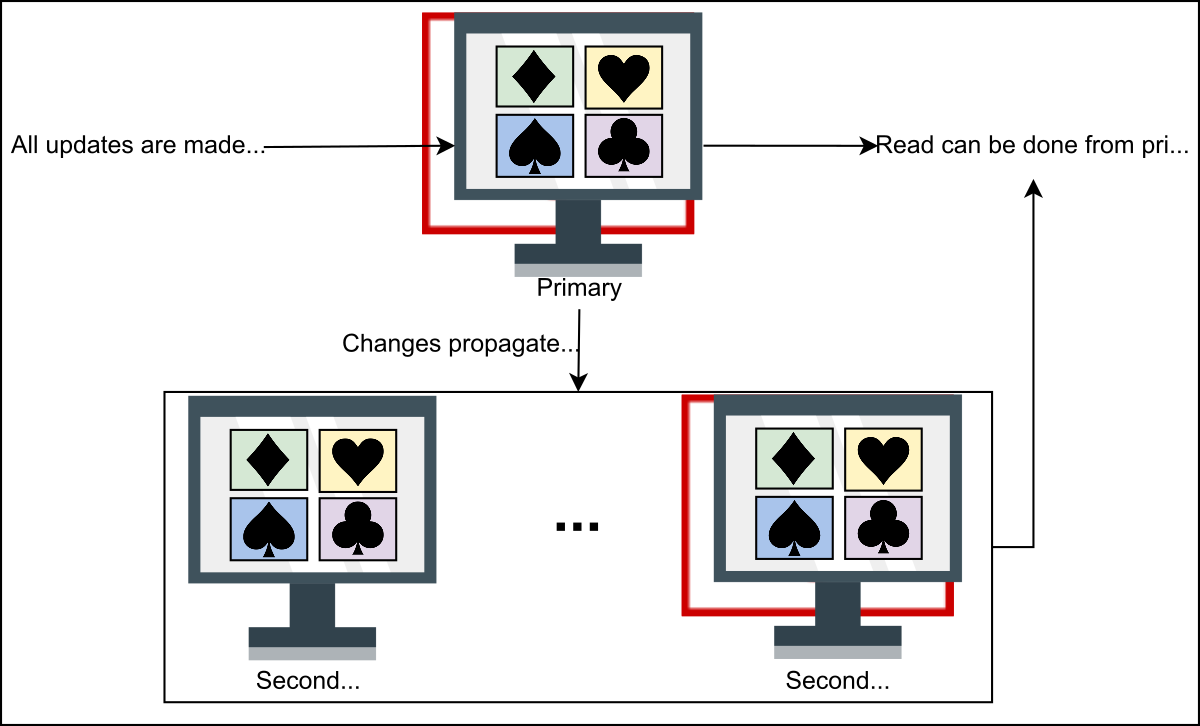
\includegraphics[width=0.5\textwidth]{Images/chapter_9/section_5241733675220992/5924227807182848.png}
 \caption{Primary-secondary data replication model where data is replicated from primary to secondary}
\end{figure}

\begin{quote}
\textbf{Quiz:}
\\
\textbf{Question 1:} What happens when the primary node fails?
\\
\textbf{Answer:} In case of failure of the primary node, a secondary node can be appointed as a primary node, which speeds up the process of recovering the initial primary node. There are two approaches to select the new primary node: manual and automatic. In a manual approach, an operator decides which node should be the primary node and notifies all secondary nodes. In an automatic approach, when secondary nodes find out that the primary node has failed, they appoint the new primary node by conducting an election known as a leader election: A leader is typically assigned based on a factor, such as choosing the processor with the highest identifier.
\end{quote}

\paragraph{Primary-secondary replication methods}\label{M4oRlp_0gzrWcyWCBkt-0}
\\
There are many different replication methods in primary-secondary replication:

\begin{itemize}
\item
\protect\phantomsection\label{SQk2F7m0y2VRKmWv_aFzN}
Statement-based replication
\item
\protect\phantomsection\label{IVpHtZ0N8fKS7qDmY9txZ}
Write-ahead log (WAL) shipping
\item
\protect\phantomsection\label{tsWl6D2xvmWWgIDayO94J}
Logical (row-based) replication
\end{itemize}
\\
Let's discuss each of them in detail.
\\
\subparagraph{Statement-based replication}\label{SUlp5J4jYvphLodGn3MiU}
\\
\textbf{Statement-based replication (SBR)} is an approach used in MySQL databases.
\\
In this approach, the primary node executes the SQL statements such as \texttt{INSERT}, \texttt{UPDATE}, \texttt{DELETE}, etc., and then the statements are written into a log fileIn many databases, transactions are captured in a file known as a log file or binlog.. In the next step, the log file is sent to the secondary nodes for execution.
\\
This type of replication was used in MySQL before version 5.1.
\\
\textbf{Best case usage:} This type of replication requires all writes to be directed through a single master node, while read-only queries can be served by any replica.
\\
For workloads that consist mostly of reads and only a small percentage of writes (a common pattern on the web), there is an attractive option to create multiple followers and distribute read requests across them. This removes a load from the leader and allows read requests to be served by nearby replicas.
\\
While this type of replication appears beneficial, it also has some drawbacks. For example, any nondeterministicUPDATE and DELETE statements that use a LIMIT clause without an ORDER BY clause are considered nondeterministic. functions such as \texttt{NOW()} might result in distinct writes on the primary and secondary nodes.
\begin{quote}
\textbf{Note:} The \texttt{NOW()} function returns the current date and time according to the system clock.
\end{quote}
\\
\subparagraph{Write-ahead log (WAL) shipping}\label{WxQCtPSGOZlG5JaJndrqZ}
\\
\textbf{Write-ahead log (WAL) shipping} is a data replication technique used in both PostgreSQL and Oracle.
\\
In this technique, when a transaction occurs, it's initially recorded in a transactional log file, and the log file is written to disk. Subsequently , the recorded operations are executed on the primary database before being transmitted to secondary nodes for execution.
\\
Unlike SBR, WAL maintains transactional logs instead of SQL statements in a log file, ensuring consistency when dealing with nondeterministic functions. Writing to disk also aids in recovery in case of crash failures.
\\
For example, when an operation like an \texttt{UPDATE} is executed in PostgreSQL, it's first written to the transactional log file and disk before being applied to the database. This entry in the transactional log can include details such as the transaction ID, operation type, affected table, and new values, after which the changes are replicated to the secondary nodes.
\\
However, the drawback of WAL is its tight coupling with the inner structure of the database engine, making software upgrades on the leader and followers complicated.
\\
\subparagraph{Logical (row-based) replication}\label{dHiCB84akT7wBW9mj9XvP}
\\
\textbf{Logical (row-based) replication} is utilized in various relational databases, including PostgreSQL and MySQL.
\\
In this approach, changes made to the database are captured at the level of individual rows and then replicated to the secondary nodes. Instead of replicating the actual physical changes made to the database, this approach captures the operations in a logical format and then executes them on secondary nodes.
\\
For example, when operations like \texttt{INSERT} or \texttt{UPDATE} are performed, the entire affected row is captured on the primary node, containing all the column values of the specified row.
\\
This captured change is then executed on secondary nodes, ensuring that the data remains consistent with the data on the primary node. It offers advantages in terms of flexibility and compatibility with various schema types.
\\
\paragraph{Common problems using asynchronous primary-secondary replication}\label{R16Bwh-0S-YSTdJrA2YTx}
\\
Asynchronous primary-secondary replication introduces certain challenges that can affect data consistency and user experience. Key issues include:

\begin{itemize}
\item
\protect\phantomsection\label{OnzEaeDyIxUd8Q-y-o4c2}
There is a chance that the new master may not receive all the writes from the old master (assuming it is still down). Hence , those write changes will be discarded, which could impact other listening applications and end clients.
\item
\protect\phantomsection\label{47stiyuqfUA246HimRuKt}
If the user attempts to read the data immediately after writing, the new data may not have been replicated yet. However, to the user, it will look as though the data they submitted was lost.
\end{itemize}
\\
\textbf{Solution:}~When reading something that the user may have modified, read it from the leader; otherwise, read it from a follower.
\\
This requires that you have some way of knowing if something has been modified without actually querying it. For example, user profile information on a social network is typically only editable by the profile owner and not by anyone else.
\\
Thus, a simple rule is to always read the user's own profile from the leader and to read any other users' profiles from a follower.
\\
\textbf{Cons:} This adds more stress to the master node.

\subsubsection{Multi-leader replication}\label{CRrrmoZeP4X019dd6DanY}
\\
As discussed above, single leader replication using asynchronous replication has a drawback.
\\
There's only one primary node, and all writes must go through it, which limits performance. In the event of the primary node\textquotesingle s failure, the secondary nodes may not have the updated database. \textbf{Multi-leader replication} is an alternative to single-leader replication.
\\
There are multiple primary nodes that process the writes and send them to all other primary and secondary nodes to replicate.
\\
This type of replication is used in databases, along with external tools such as the Tungsten Replicator for MySQL. This kind of replication is particularly useful in applications where we can continue working even when offline---for example, a calendar application that allows us to schedule meetings even without internet access.
\\
Once we're online, it replicates its changes from our local database (our mobile phone or laptop acts as a primary node) to other nodes.

\begin{figure}[htbp]
 \centering
 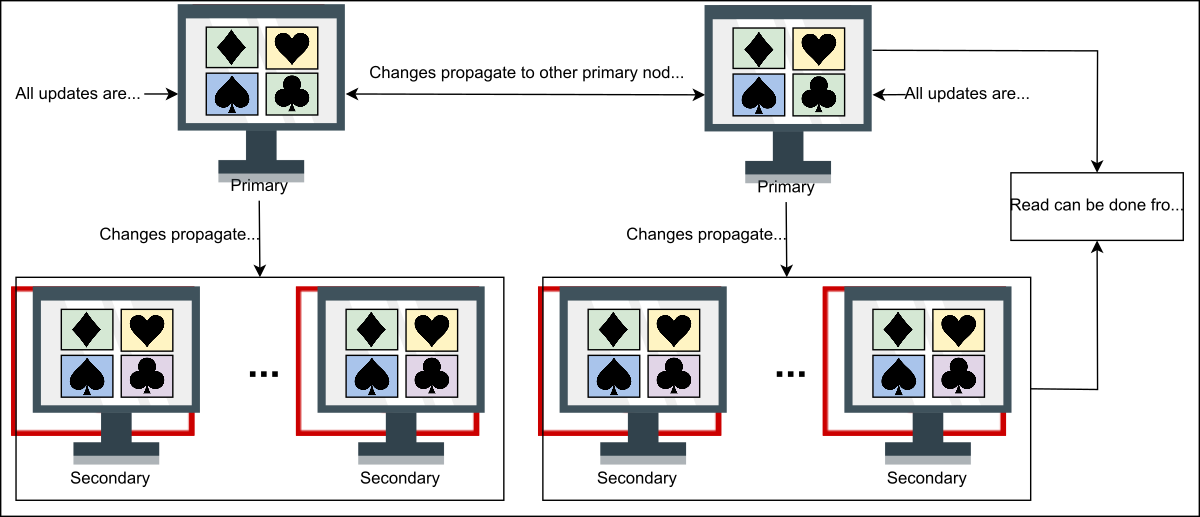
\includegraphics[width=0.5\textwidth]{Images/chapter_9/section_5241733675220992/5552567090413568.png}
 \caption{Multi-leader data replication model (all-to-all topology)}
\end{figure}

\textbf{Common data distribution/migration pattern}

\begin{itemize}
\item
\textbf{Bi-direction:} Reporting instance
\item
\textbf{Unidirectional:} Instant fail-over (Multi-leader replication)
\item
\textbf{Peer-to-peer:} Load balancing (High Availability)
\item
\textbf{Broadcast:} Wide-level data distribution to multiple instances
\item
\textbf{Consolidation:} Data warehouse (data storage)
\end{itemize}
\\
\paragraph{Conflict}\label{PzqAJX4o66ZS_XoonFcaH}
\\
Multi-leader replication gives better performance and scalability than single-leader replication, but it also has a significant disadvantage.
\\
Since all primary nodes concurrently handle write requests, they may modify the same data, potentially creating a conflict between them. For example, suppose the same data is edited by two clients simultaneously. In that case, their writes will be successful in their associated primary nodes, but when they reach the other primary nodes asynchronously, it creates a conflict.
\\
\paragraph{Handle conflicts}\label{KyIqzBZtuN_iGmoyXvnPt}
\\
Conflicts can result in different data at different nodes. These should be handled efficiently without losing any data. Let 's discuss some of the approaches to handling conflicts:

\begin{figure}[htbp]
 \centering
 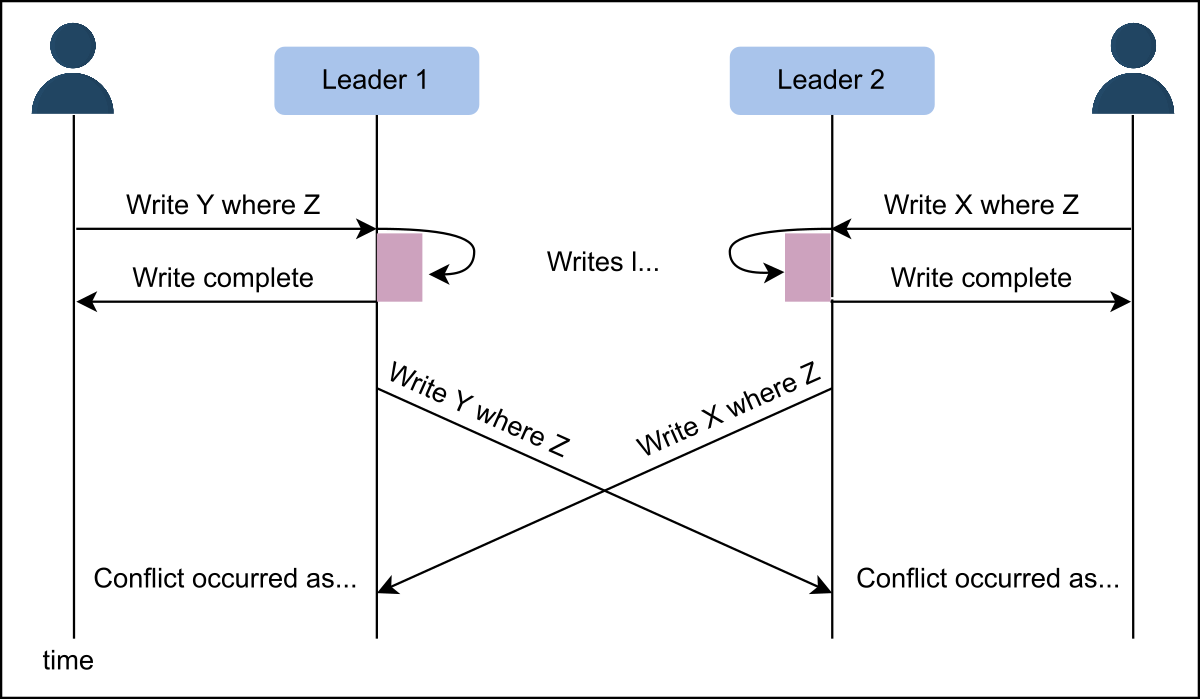
\includegraphics[width=0.5\textwidth]{Images/chapter_9/section_5241733675220992/6509582298120192.png}
 \caption{Conflict of writes}
\end{figure}

\subparagraph{Conflict avoidance}\label{RrlEvY2LC0_iMpj_fvCKD}
\\
A simple strategy to deal with conflicts is to prevent them from happening in the first place.
\\
Conflicts can be avoided if the application can verify that all writes for a given record are routed through the same leader. However, the conflict may still occur if a user moves to a different location and is now near a different data center.
\\
If that happens, we need to reroute the traffic. In such scenarios, the conflict avoidance approach fails, resulting in concurrent writes.
\\
\subparagraph{Last-write-wins}\label{LzKP9dCVigj4ML9raycAn}
\\
Using their local clock, all nodes assign a timestamp to each update.
\\
When a conflict occurs, the update with the latest timestamp is selected. This approach can also create difficulty because the clock synchronization across nodes is challenging in distributed systems. There 's a clock skew that can result in data loss.
\\
\subparagraph{Custom logic}\label{jBSEvQ5WMSxuoh2qBu1Wb}
\\
In this approach, we can write our own logic to handle conflicts according to the needs of our application. This custom logic can be executed on both read and write operations. When the system detects a conflict, it calls our custom conflict handler.
\\
\paragraph{Multi-leader replication topologies}\label{8ZwbqOAgTbJQjoUtU0Prs}
\\
There are several topologies through which multi-leader replication is implemented, including the circular topology, star topology, and all-to-all topology.
\\
The most common is the all-to-all topology. In a star and circular topology, there's again a similar drawback that if one of the nodes fails, it can affect the whole system. That 's why all-to-all is the most used topology.

\subsubsection{Peer-to-peer/leaderless replication}\label{II-0xD6RiqVyVtslSa3r6}
\\
In primary-secondary replication, the primary node is a bottleneck and a single point of failure.
\\
Moreover, it helps to achieve read scalability but fails to provide write scalability. The \textbf{peer-to-peer replication} model resolves these problems by eliminating the need for a single primary node. All nodes have equal weight and can accept both read and write requests.
\\
This replication scheme is stored in the Cassandra database.

\begin{figure}[htbp]
 \centering
 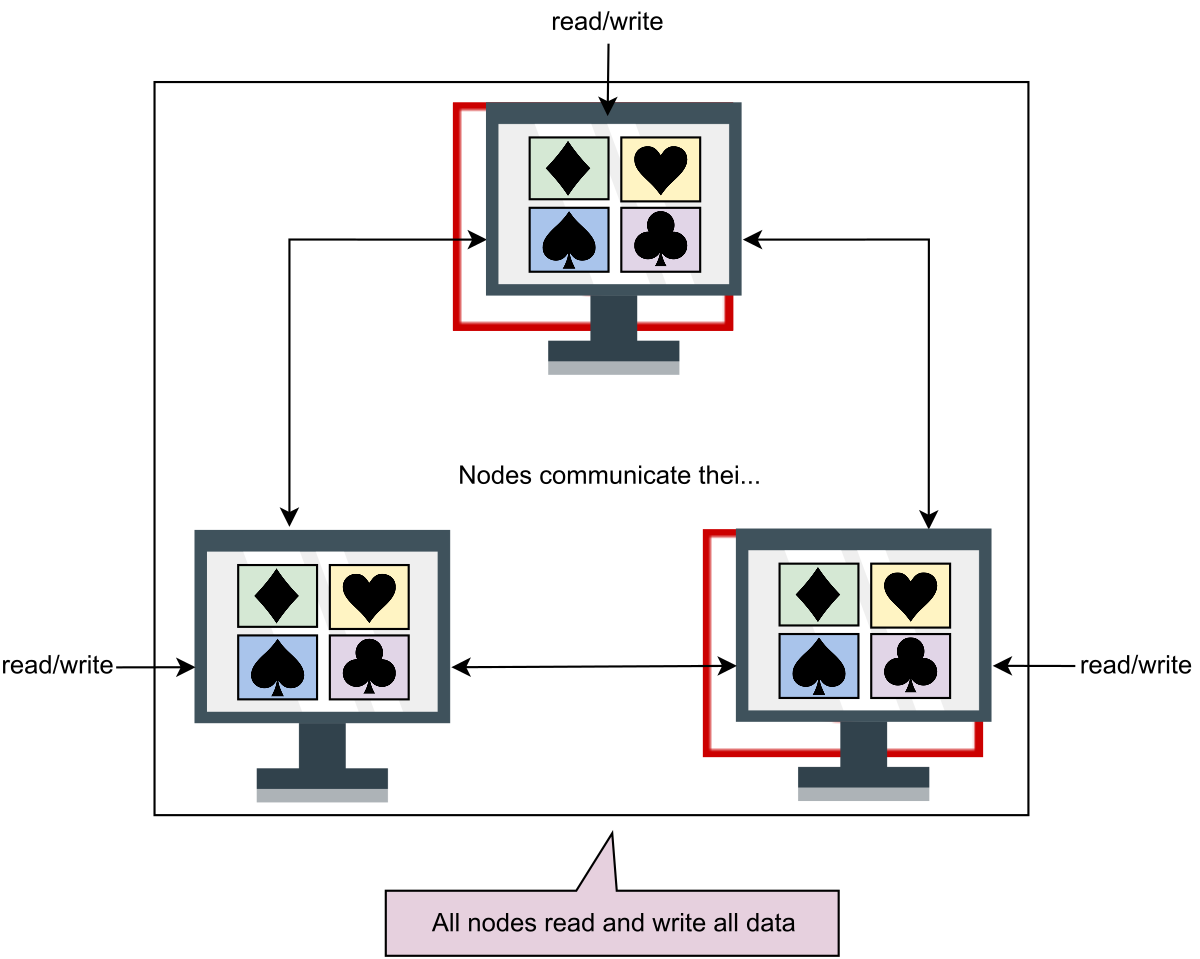
\includegraphics[width=0.5\textwidth]{Images/chapter_9/section_5241733675220992/6122582969679872.png}
 \caption{Peer-to-peer data replication model where all nodes apply reads and writes to all the data}
\end{figure}

Like primary-secondary replication, this replication can also yield inconsistency. This is because when several nodes accept write requests, it may lead to concurrent writes. A helpful approach used for solving write-write inconsistency is called \textbf{quorums}.
\\
\paragraph{Quorums}\label{9-8B2Kza_yFRBqyvsOXUv}
\\
Let's suppose we have three nodes.
\\
If at least two out of three nodes are guaranteed to return successful updates, it means only one node has failed. This means that if we read from two nodes, at least one of them will have the updated version, and our system can continue working.
\\
If we have \protect\phantomsection\label{katex_inline_X1ClQkdrTTu5n4AZmUCrK}{{{\(n\)}}} nodes, then every write must be updated in at least \protect\phantomsection\label{katex_inline_b_6Yk9JJaIO8b380TkQvg}{{{\(w\)}}} nodes to be considered a success, and we must read from \protect\phantomsection\label{katex_inline_Sv-bCRejjWdjYQgQMfhxP}{{{\(r\)}}} nodes.
\\
We'll get an updated value from reading as long as \protect\phantomsection\label{katex_inline_oiUnrfqbTVTtOReKs03CR}{{{\(w+r> n\)}}} because at least one of the nodes must have an updated write from which we can read. Quorum reads and writes adhere to these \protect\phantomsection\label{katex_inline__FY2p9rZxG9kdCm0S0YCt}{{{\(r\)}}} and \protect\phantomsection\label{katex_inline_G-E-7zuhuJItOvRVzeBh5}{{{\(w\)}}} values. These
\protect\phantomsection\label{katex_inline_l4jLKkjGbZbZjnA4s58o_}{{{\(n\)}}}, \protect\phantomsection\label{katex_inline_AsZVwOCzmx7yfpCcNwMxs}{{{\(w\)}}}, and \protect\phantomsection\label{katex_inline_0bg4Oa90Daq7QepdqwOfG}{{{\(r\)}}} are configurable in Dynamo-style databases.

\begin{figure}[htbp]
 \centering
 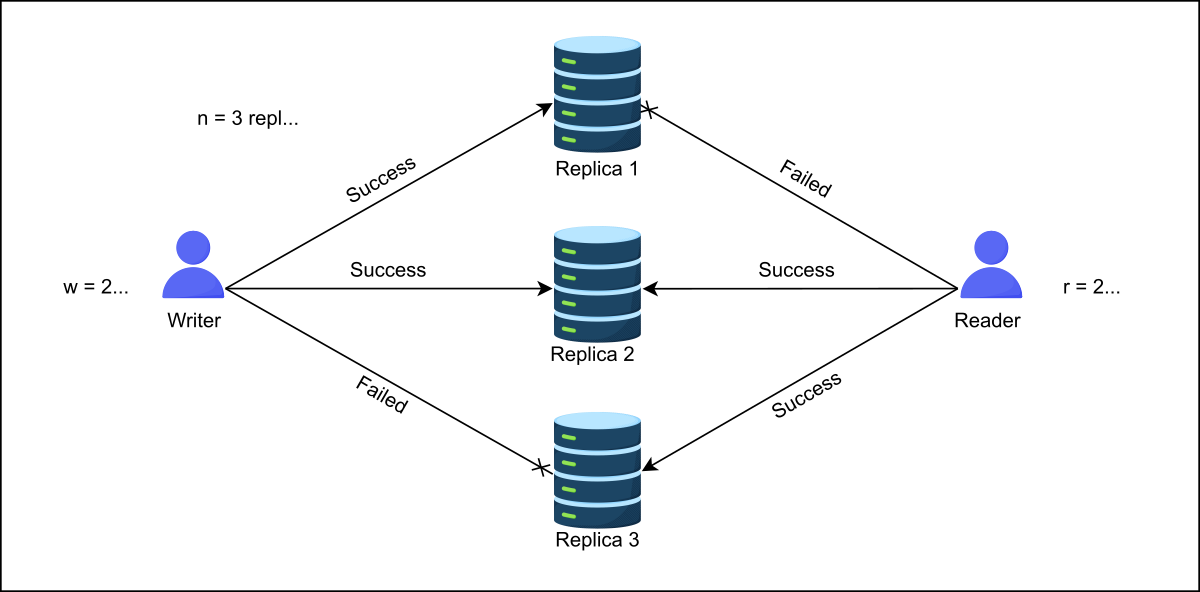
\includegraphics[width=0.5\textwidth]{Images/chapter_9/section_5241733675220992/6626127471050752.png}
 \caption{Reader getting an updated value from replica 2}
\end{figure}

\begin{quote}
For more details on the topic of Quorum, refer to these links:

\begin{itemize}
\item
\href{https://www.educative.io/answers/what-is-a-quorum}{What is Quorum?}
\item
\href{https://www.educative.io/answers/what-is-quorum-in-distributed-systems}{What is Quorum in distributed systems?}
\end{itemize}
\end{quote}

\subsection*{Quiz}
\vspace{0.3cm}
\noindent
\textbf{Question 1:} Which replication mechanism is the most appropriate (high throughput, low latency to client, low implementation overhead) when our workload is read-heavy?
\\[0.2cm]
\begin{itemize}
 \item \textbf{[CORRECT]} Primary-secondary/single leader replication
\\[0.1cm]
\textit{Explanation:} 
Primary-secondary/single leader replication is best suited for read-heavy workloads since multiple secondaries can serve reads with low latency and minimal complexity.
 \item Multi-leader replication
\\[0.1cm]
\textit{Explanation:} 
Multi-leader replication increases write availability but adds conflict resolution overhead, which is unnecessary for primarily read-heavy workloads.
 \item Peer-to-peer replication
\\[0.1cm]
\textit{Explanation:} 
Peer-to-peer replication is fully decentralized but complex to implement and coordinate, offering little benefit over simpler leader-based setups for read-heavy scenarios.
\end{itemize}

% End of section content